\chapter{Application on real data}
In the simulation study in the previous chapter, we contrasted the fixed intercept version and the updating intercept version of FHTBoost.
In general, FHTBoost seems to provide a decent model for correlated, realistic survival data, with average difference of deviance much smaller than 0, meaning that including covariates in the model increases its fit to test data.
We now evaluate the performance of FHTBoost on a real data example.
Specifically, we consider data from \citet{oberthuer-data}, consisting of data from patients diagnosed with neuroblastoma.
The dataset includes a relatively small number of patients, with information on two clinical covariates and around 10 000 gene expressions.
We use FHTBoost on this data to estimate an FHT model, and assess the model fit with deviance.
Finally, we compare the predictive power of FHTBoost to CoxBoost via the Brier score (section \ref{sec:brier}), which is a method to estimate a Cox regression model using a boosting framework (see, e.g., \citet{BinderSchumacher2008}).

\section{Neuroblastoma}
We consider survival data from \citet{oberthuer-data}, consisting of patients diagnosed with neuroblastoma.
Neuroblastoma is a malignant pediatric tumor that accounts for about 8\% of all childhood cancers.
One of the hallmarks of the disease is its contrasting biological behavior, which results in diverse clinical courses ranging from spontaneous regression to rapid and fatal tumor progression despite intensive treatment.

In recent years, several markers have been reported to offer valuable prognostic information.
These markers are routinely determined by the current German neuroblastoma clinical trial NB2004 to stratify patients into groups of high risk (50\%) or low risk (50\%) of disease.
Therapeutic strategies vary according to these risk categories, and they range from a wait-and-see approach for those in the low risk group
to intensive treatment for the high-risk group.
However, common clinical experience suggests that such risk classification is still suboptimal for a substantial number of patients.

Originally, the data consist of two separate data sets:
A larger training set, collected in Germany, and a smaller test set, collected in several countries.
The training set consists of 256 patients of the German Neuroblastoma Trials NB90-NB2004, where the patients were diagnosed between 1989 and 2004.
The test set is an independent set of 120 patients from national trials in several countries (including 29 from Germany).
Due to a low number of events in the NB2004 low risk group, and following \citet{bovelstad2009}, we merge the ``training set'' and the ``test set'' into one data set.
Hence, in total, the data consists of 362 patients suffering from neuroblastoma.
There are 9978 gene expressions measurements, comprised of those measurements that are in probes from both the ``training set'' and the ``test set.''
From each patient, we have information on their risk group according to the current German neuroblastoma trial, as well as the patient's age at diagnosis.
In this data set, 89 out of the 362 observations have missing values.
We remove all of these observations, and are left with a data set of 273 individuals with full observations.
Finally, for each individual we have the possibly censored event time, which in the case of an event is the time to a fatality, in years from diagnosis.
The median follup-up time without a fatal event was 4.14 years.
42 of the 273 children experienced a fatal event within the follow up, which is a proportion of 31.5\%.
Of these, 86 children were classified as having high-risk, while the remaining 187 were not.
The risk indicator is coded as a binary variable, where low risk is coded as 0, and high risk as 1.

Due to the lack of data, \citet{bovelstad2009} generated 50 random splits of training and test sets from the merged data set.
We do the same, only we generate 100 random splits.
First, however, we report the analysis of one single (the first) split of train and test data, to show how to interpret the results.

\section{A single split of the data set}
The data are split in a training set (2/3) and test set (1/3), stratified by the event status.
The training set consists of 182 patients, where 28 are observed events.
The test set consists of 91, where 14 are observed events.

\subsection{Cross-validation on training set}
As has been shown previously, cross-validation should be repeated with different division of folds, as this reduces variance in the estimate of $\mstop$.
We therefore perform a (10 times) repeated 5-fold cross validation to find the optimal number of iterations.
Note in Figure \ref{fig:neuroblastoma-cv} the impact of running the cross-validation in a repeated fashion:
We would not have selected the same $\mstop$ in all of these 10 single 5-fold cross-validations.
%We first performed a 10-fold repeated cross-validation, but this parameter search did not converge, i.e., the log-likelihood kept increasing.
%Upon further inspection, we found that one of the folds was the main cause of this, as the log-likelihood for that particular fold continued to increase, even after 400 iterations, while the other folds were in overfitting territory.
%We concluded that splitting a training set of around 180 into 10 folds would eventually cause a problem in one of the folds, as there was too little information left.
We find $\mstop=20$ to be optimal, i.e., the minimizing iteration number, shown as the red vertical line in Figure \ref{fig:neuroblastoma-cv}.
Each dotted gray line in the figure is the sum of the negative log-likelihood of a model trained on 4 folds and applied to the last fold, as a function of the iteration number $m$, i.e. the cross-validated test error.
The solid black line is the mean of these 10 gray lines, and it is this line that we choose the minimizer of.
As we can see, in this example the boosting algorithm, in contrast to the original AdaBoost, eventually overfits, so it is important to select the number of boosting steps by cross-validation.

\begin{figure}
\caption{
    Repeated 5-fold cross validation on training set generated from neuroblastoma data set \citep{oberthuer-data}.
    The grey lines refer to the cross validation error for a single 5-fold CV implementation,
    the black line is the average of 10 such replications.
    The red vertical line highlights the best value for the number of boosting steps.
}
\label{fig:neuroblastoma-cv}
\centering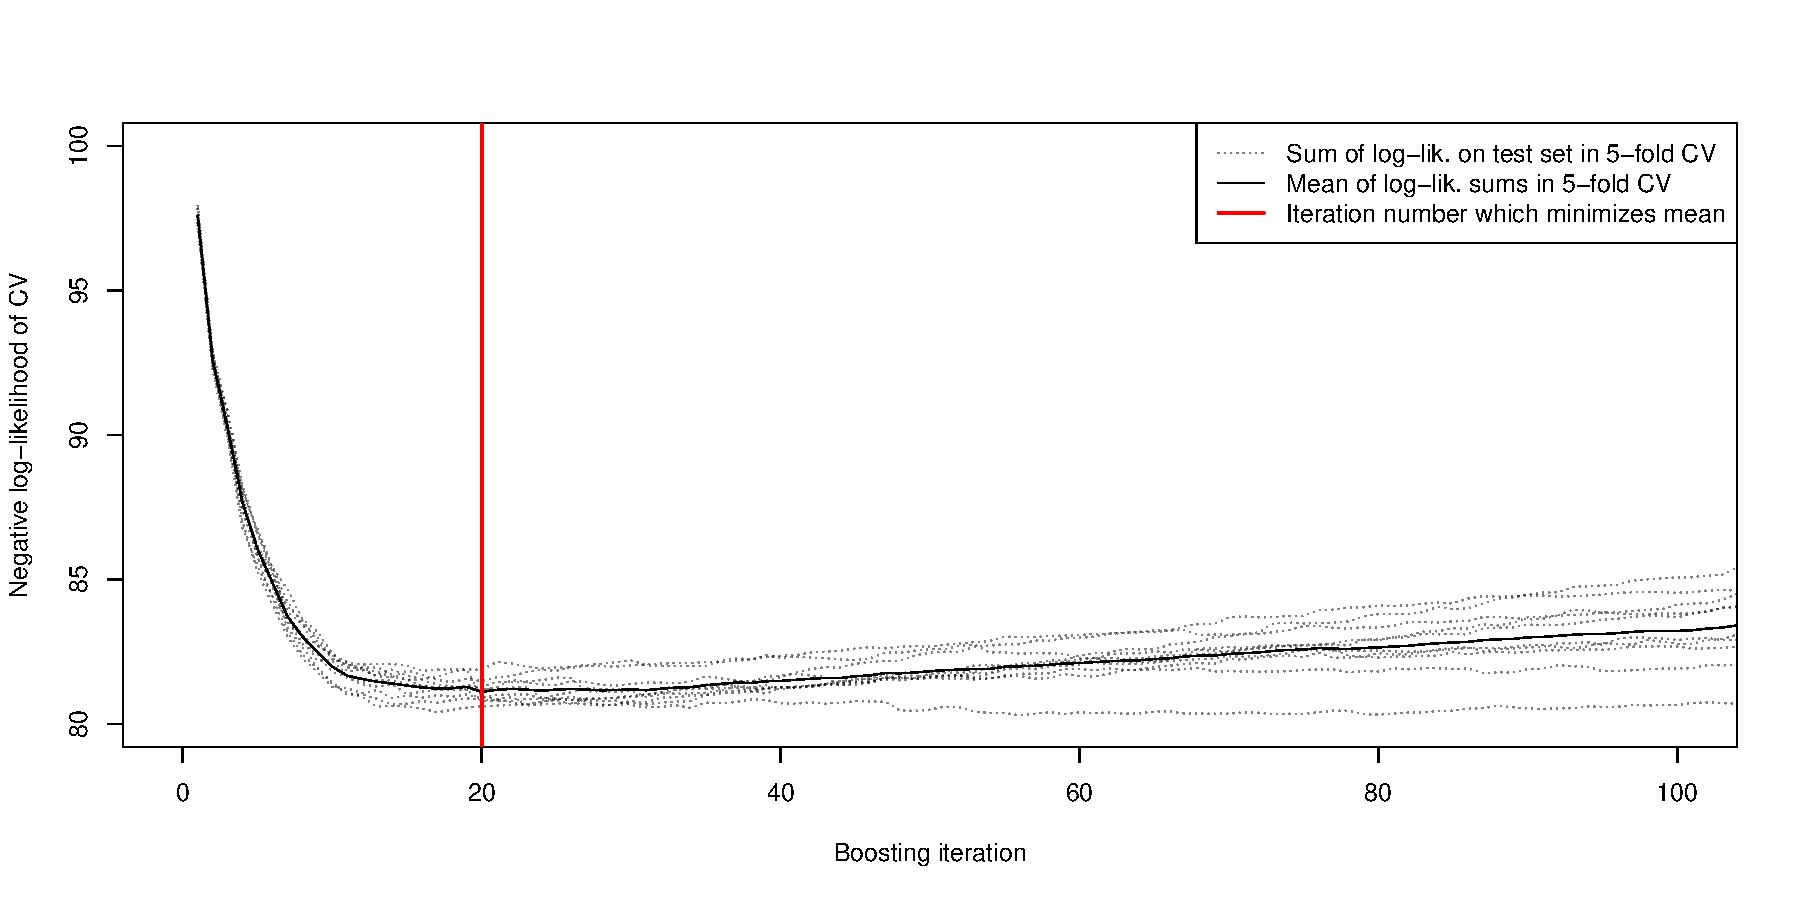
\includegraphics[scale=0.4]{example_cv_loglik.pdf}
\end{figure}

\subsection{Results}
We run the FHTBoost algorithm with a fixed intercept for $\mstop$ iterations, resulting in an estimated model.
We now discuss the results of this model.

\begin{table}
\caption{Estimated FHT null model on a single split of the neuroblastoma data set \citep{oberthuer-data}}
\label{tab:neuroblastoma-intercepts}
\centering
\begin{tabular}{lr}
\toprule
Intercept  & Value\\
\hline
$\hat{\beta}_0$ & 0.692 \\
$\hat{\gamma}_0$ & 0.077 \\
\bottomrule
\end{tabular}
\end{table}

\subsubsection{Null model interpretation}
We recall the concept of a null model, which is a model without covariates.
In an FHT context with a Wiener process, this means a model with initial level
\begin{equation*}
    \hat{y}_0^{[0]}=\exp\left(\hat{\beta}_0\right)
\end{equation*}
and drift
\begin{equation*}
    \hat{\mu}^{[0]}=\hat{\gamma}_0.
\end{equation*}
We first look at the intercepts, reported in Table \ref{tab:neuroblastoma-intercepts}, basically the parameters of the null model.
The estimated intercept for the gene data, $\hat{\beta}_0$, is 0.692.
Remember that the vector $\bbeta$ corresponds to the initial level $y_0$ of the health process, through the log link function.
The null model, without any covariate effects, therefore has a $y_0$ of $\exp(0.692)=1.998$.
The intercept $\gamma_0$ corresponding to the clinical data is estimated to be 0.077.
Since these are related by identity link, the drift $\mu$ is then also 0.077.
This means that the health process with the FHT interpretation that arises from our estimation is a Wiener process with a relatively small initial level of 1.998, and with a \textit{positive} drift, albeit slightly, of 0.077.
We further recall from section \ref{subsec:wiener} that a Wiener process $W(t)$ has variance equal to its time $t$.
%It is therefore quite probable that an FHT process with initial level $1.998$ and drift $0.077$ will cause an event.
The large variability of the process relative to its starting point means there is still a significant chance of recurrence of neuroblastoma.
The resulting health process is
\begin{equation*}
    Y(t)=1.998+W(t)\cdot0.077t,
\end{equation*}
where $W(t)\sim N(0,\sqrt{t})$,
i.e.,
\begin{equation*}
    Y(t)\sim N(1.998+0.077t,\sqrt{t}).
\end{equation*}
To get a feeling of the variability of $Y(t)$, and potential trajectories of such a process, we plot 10 realizations of this process in Figure \ref{fig:neuroblastoma-wien}.
Of these particular 10 processes, 4 processes at some point go below 0.
These are given a red color in figure \ref{fig:neuroblastoma-wien}.
In the FHT interpretation, then, these health processes would cause a fatal event of the child.
To get a better estimate of the proportion of health processes not hitting the death state, we need to sample more processes.
We sampled 10000, and 4695 of these went below 0 within $t=12$, i.e., a proportion of 0.531 did not experience a fatal event.
In section \ref{sec:FHT}, specifically in equation \eqref{eq:P-inf-FHT}, we gave the probability of an IG FHT lifetime not ending, i.e., the cure rate.
We will have a non-zero cure rate if the drift is positive, like we have here in our estimated null model.
We calculate its cure rate, obtaining
\begin{align*}
    \Pr{(T=\infty)}=1-\Pr{(T<\infty)}&=1-\exp{(-2\cdot y_0^{[0]}\cdot\mu^{[0]})}\\
    &=1-\exp{(-2\cdot 1.998\cdot 0.077)}=0.265,
\end{align*}
meaning about three in four should have a recurrence during their lifetime.
For this training set, 28 out of 182 are observed events, meaning only 0.154 have experienced a fatal event.
Note that this is with a medium follow-up on patients of 4.5 years, while we simulated the paths of all processes for 12 years.
It is still a bit off from the cure rate obtained from the estimated null model, but our model does predict a non-zero cure rate.
\begin{figure}
\caption{Curves for 10 randomly generated Wiener processes with parameters $y_0=1.998$ and $\mu=0.077$, corresponding to the estimated null model from the neuroblastoma data set \citep{oberthuer-data}.}
\label{fig:neuroblastoma-wien}
\centering
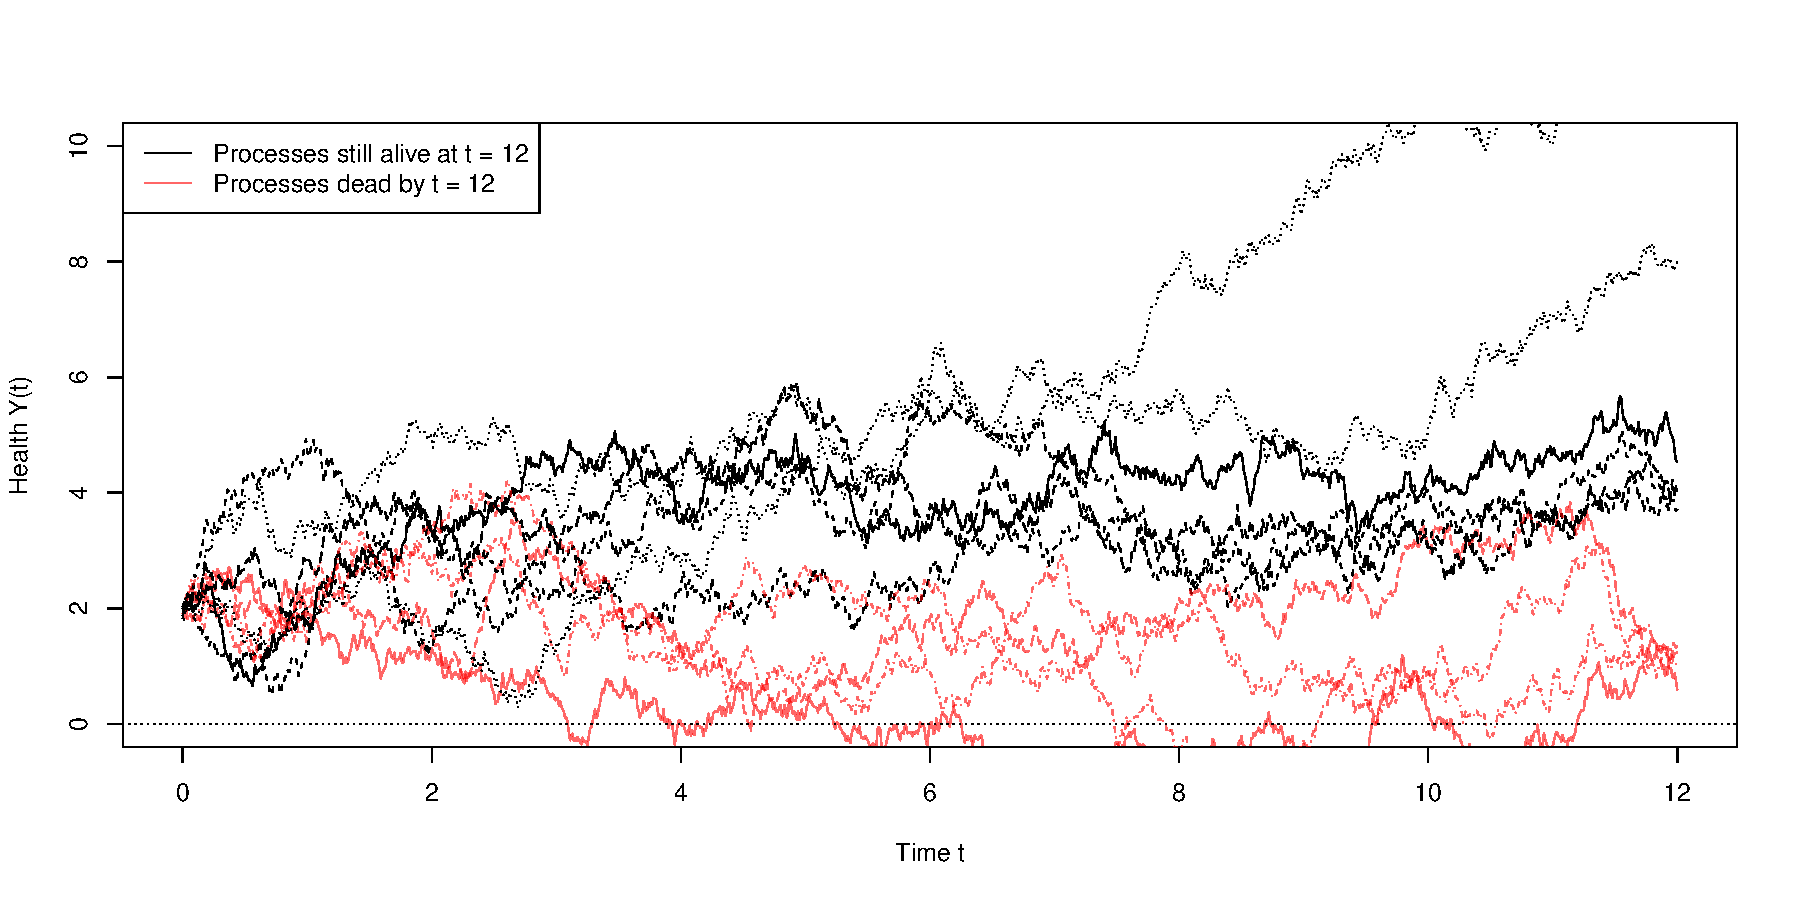
\includegraphics[scale=0.4]{example_wieners6.pdf}
\end{figure}

Consider the fact that the initial level $y_0$ is quite low.
Since we are looking at when, if ever, a neuroblastoma patient will have a fatal event after diagnosis, this initial level of the Wiener process is the health level of a patient \textit{at} its diagnosis.
The health of such a child is presumably quite precarious, as neuroblastoma is a malignant cancer.
Therefore it makes sense that the initial level $y_0$ of the child's health process is quite low.
Furthermore, the fact that the drift $\mu$ is positive also makes sense.
Since the individuals in the study are young children, and we are looking at a timeframe that does not comprise the length of a typical human life, the health level of most children should indeed increase after diagnosis.
However, as mentioned, and as clinicians experience, the survival probability of patients vary, even among those specified as high-risk.
We therefore must look at estimated covariates to see if we can understand this variability.

\subsubsection{Estimated covariate effects}
Let us further look at estimated covariate effects in Table \ref{tab:oberthuer-gamma} and Table \ref{tab:oberthuer-beta}.
We first observe that the boosting algorithm has included both clinical covariates into the model, i.e. the age at diagnosis and the risk indicator.
The model has also included 8 genes for this training data set.
Remember that we centered each column of the covariate matrices, such that the mean across all individuals is (approximately) 0 for each covariate $j$.
%\begin{equation}
%    \overline{x}_j=\frac{1}{n}\sum_{i=1}^n x_{i,j}\approx 0,
%\end{equation}
%\begin{equation}
%    s_j=\frac{1}{n}\sum_{i=1}^n (x_{i,j}-\overline{x}_j)^2\approx 1.
%\end{equation}
%(See a previous section for an explanation of why centering and scaling is important.)
For the gene expressions, this is not particularly important with regards to interpretation, as the scale of these do not lend themselves easily to interpretation.
However, to properly consider the interpretation of the estimated parameters for to the clinical measurements, we should consider these on their original scale.
For example, the covariate corresponding to risk, namely $\gamma_1$, is originally either 0 or 1, depending on the covariate.
After standardizing, these are -0.677 and 1.472, respectively.
The most striking result here is the large parameter corresponding to risk.
We calculate the drift parameter for those individuals designated as high-risk, and it is
\begin{equation*}
    \mu^{[0]}_{\text{high-risk}}=0.077-0.189\cdot1.472=-0.202.
\end{equation*}
Whereas for those designated as low and intermediate risk, it is
\begin{equation*}
    \mu^{[0]}_{\text{low-risk}}=0.077-0.189\cdot-0.677=0.205.
\end{equation*}
In other words the drift for those with high risk is \textit{negative}, while it is \textit{positive} for low risk.
Since age is standardized, these two drift covariates are the mean drift parameters for each of the groups.
We can first check to see if this holds true for all individuals within the risk groups.
The effect of age is negative, which means that there is some downward effect on the drift as the child's age increases.
This negative effect could also potentially lead to low-risk individuals having an estimated negative drift, if the child is sufficiently old.
This is, however, not the case.
The effect of age is so small as to not impact the sign of the drift.
Because the maximum standardized age is 4.193, the age contribution to drift is bounded below by 
\begin{equation*}
    -0.029\cdot4.193=-0.122.
\end{equation*}
Similarly, there are no high-risk individuals for which the drift will be positive, since the minimum standardized age is -0.724, and so the effect of age is bounded above by
\begin{equation*}
    -0.029\cdot0.724=0.021.
\end{equation*}
Hence, crucially, this means that the model predicts that \textit{all} high-risk individuals will eventually have a recurrence of neuroblastoma cancer.
This seems to resonate with the fact that these children are indeed characterized as having a high risk of recurrence.
Those not designated as high-risk, on the other hand, have a non-zero probability of not experiencing recurrence.
We calculate it using the formula seen previously, namely
\begin{equation*}
    1-\exp{(-2\cdot y_{0}^{[0]}\cdot\mu_{\text{low-risk}}^{[0]})}=1-\exp{(-2\cdot 1.998\cdot 0.205)}=0.559.
\end{equation*}
We should therefore expect, based on the estimated model, that more than half of the low-risk patients should recover.
We should also consider the gene covariates.

\begin{table}
\caption{Results of estimated clinical coefficients on neuroblastoma data \citep{oberthuer-data}.}
\label{tab:oberthuer-gamma}
\centering
\begin{tabular}{lrr}
\toprule
Clinical covariate & $\hat{\gamma}_j$ (full) & $\hat{\gamma}_j$ (clinical only)\\
\hline
Risk      &  -0.189  &  -0.268\\
Age       &  -0.029  &       0 \\
\bottomrule
\end{tabular}
\end{table}

We observe that 8 genes have been selected in 20 boosting iterations (see the $\hat{\beta}_j$ column in Table \ref{tab:oberthuer-beta}).
Some effects are estimated to be positive, some to be negative, but all are roughly the same size in absolute terms.
Again, the gene expression measurements have been centered and scaled.
However, a larger parameter does not necessarily mean that the effect of this gene is in general larger than others, as it still depends somewhat on the distribution of these.
We recall e.g. from the simulation chapter that the effect of a change in $\beta_j$ is multiplicative in $\exp(\beta_j)$, and not additive.
We might for example look at gene 6701.
The estimated effect of it is $\hat{\beta}_{6701}=0.015$.
The maximum gene effect after standardization of this gene is 3.8.
For a hypothetical observation which has mean values for all genes, and thus no effect of those, but with max effect of this gene, its $\hat{y}_{0}$ will be
\begin{equation*}
    \hat{y}_{0}=\hat{y}_0^{[0]}\cdot\exp(0.015\cdot3.8)=1.998\cdot1.09=2.115,
\end{equation*}
whereas the null model has an initial level of 1.998.
\todo[inline]{Say more?}

\begin{table}
\caption{Results of estimated gene coefficients on neuroblastoma data \citep{oberthuer-data}.}
\label{tab:oberthuer-beta}
\centering
\begin{tabular}{lrr}
\toprule
Gene $j$      & $\hat{\beta}_j$ (full) & $\hat{\beta}_j$ (genomic only)\\
\hline
Gene 49   & -0.010  &      0  \\
Gene 1447 & -0.069  & -0.047  \\
Gene 3191 &      0  & -0.051  \\
Gene 2442 &  0.012  &      0  \\
Gene 4447 &      0  & -0.062  \\
Gene 5307 &      0  &      0  \\
Gene 5527 & -0.073  & -0.098  \\
Gene 5725 & -0.009  &      0  \\
Gene 6532 & -0.011  &      0  \\
Gene 6701 &  0.015  &      0  \\
Gene 6901 &  0.011  &      0  \\
\bottomrule
\end{tabular}
\end{table}
\todo[inline]{Check Riccardo's comments on table here}

\begin{table}
\caption{Difference of deviance with FHTBoost with a fixed intercept, on a single split of the neuroblastoma data \citep{oberthuer-data}.}
\label{tab:deviances}
\centering
\begin{tabular}{lr}
\toprule
Boosting type & Difference of deviance \\
\hline
Full & -95.2 \\
Clinical ($y_0$) only  & -14.5 \\
Genomic ($\mu$) only & -104.4 \\
\bottomrule
\end{tabular}
\end{table}

\section{Comparing a clinical-genetic model to clinical-only and genetic-only models}
\citet{bovelstad2009} analysed the neuroblastoma data and compared different statistical methods to combine clinical and genomic data in Cox models.
As mentioned in subsection \ref{subsec:FHT-combine}, the FHT model lends itself easily to combining genomic and clinical data, and this holds for FHTBoost as well.
There is also a straightforward way to only use one kind of covariates, i.e., only clinical covariates or only genetic covariates.
To do this, we can use the cyclical version of the algorithm, where we boost both parameters in each step, but each has its own tuning parameter.
This lets us fix the number of boosting steps of the parameter not to be boosted to 0.
In other words, we make a genomic version of FHTBoost, or $y_0$-only version of FHTBoost, by only boosting the initial level $y_0$.
This version of FHTBoost has $m_{\text{stop},1}$, corresponding to $\mu$, fixed at 0, while we perform cross-validation in the usual way to find the optimal $m_{\text{stop},2}$, corresponding to $y_0$.
Similarly, the clinical version fixes $m_{\text{stop},2}$ at 0, and tunes the other, $m_{\text{stop},1}$, corresponding to $\mu$.
In this way, we can compare the performance of our model across the genetic and clinical data, in a similar way as in \citet{bovelstad2009}.

We do the estimation and the test set calculation, and we get the difference of deviance results shown in Table \ref{tab:deviances}.
We see here, in fact, that in this specific case the full model is beaten by the genomic model, with difference of deviance of -95.2 and -104.4, respectively.

Furthermore, we calculate the Brier scores (Section \ref{sec:brier}) of these models on each observation in the test set, see Figure \ref{fig:brier-FHT}.
Interestingly, the full FHT model is quite consistently better than the genomic model, i.e. it is better per observation in the Brier score, even though it achieves a worse difference of deviance.
It is interesting to note that these two different models perform best on each their criterion.
Furthermore, the Brier score of the full FHT model is equal to the clinical one in some parts, except in the middle, from 3 to 7 years, where it is somewhat better.
It is perhaps easiest to compare the performance if we have a number, and we get that by calculating the integrated Brier score, explained in subsection \ref{subsec:integrated-brier}, and which is effectively the average Brier score over a given range of time, in this case the times from the entire test set.

We find that the integrated Brier score for the full FHT model is 0.0679, while the estimated FHT null model achieves 0.1226, which is almost the double.
Note, however that large part of the additional error refers to the right part of the error curve (see Figure \ref{fig:brier-FHT}), where the computations are more unstable due to the reduced number of events (larger proportion of censored data).
And the genomic model attains an integrated Brier score of 0.1015, while the clinical attains 0.0708.

\begin{figure}
\caption{Brier scores for FHT models.}
\label{fig:brier-FHT}
\centering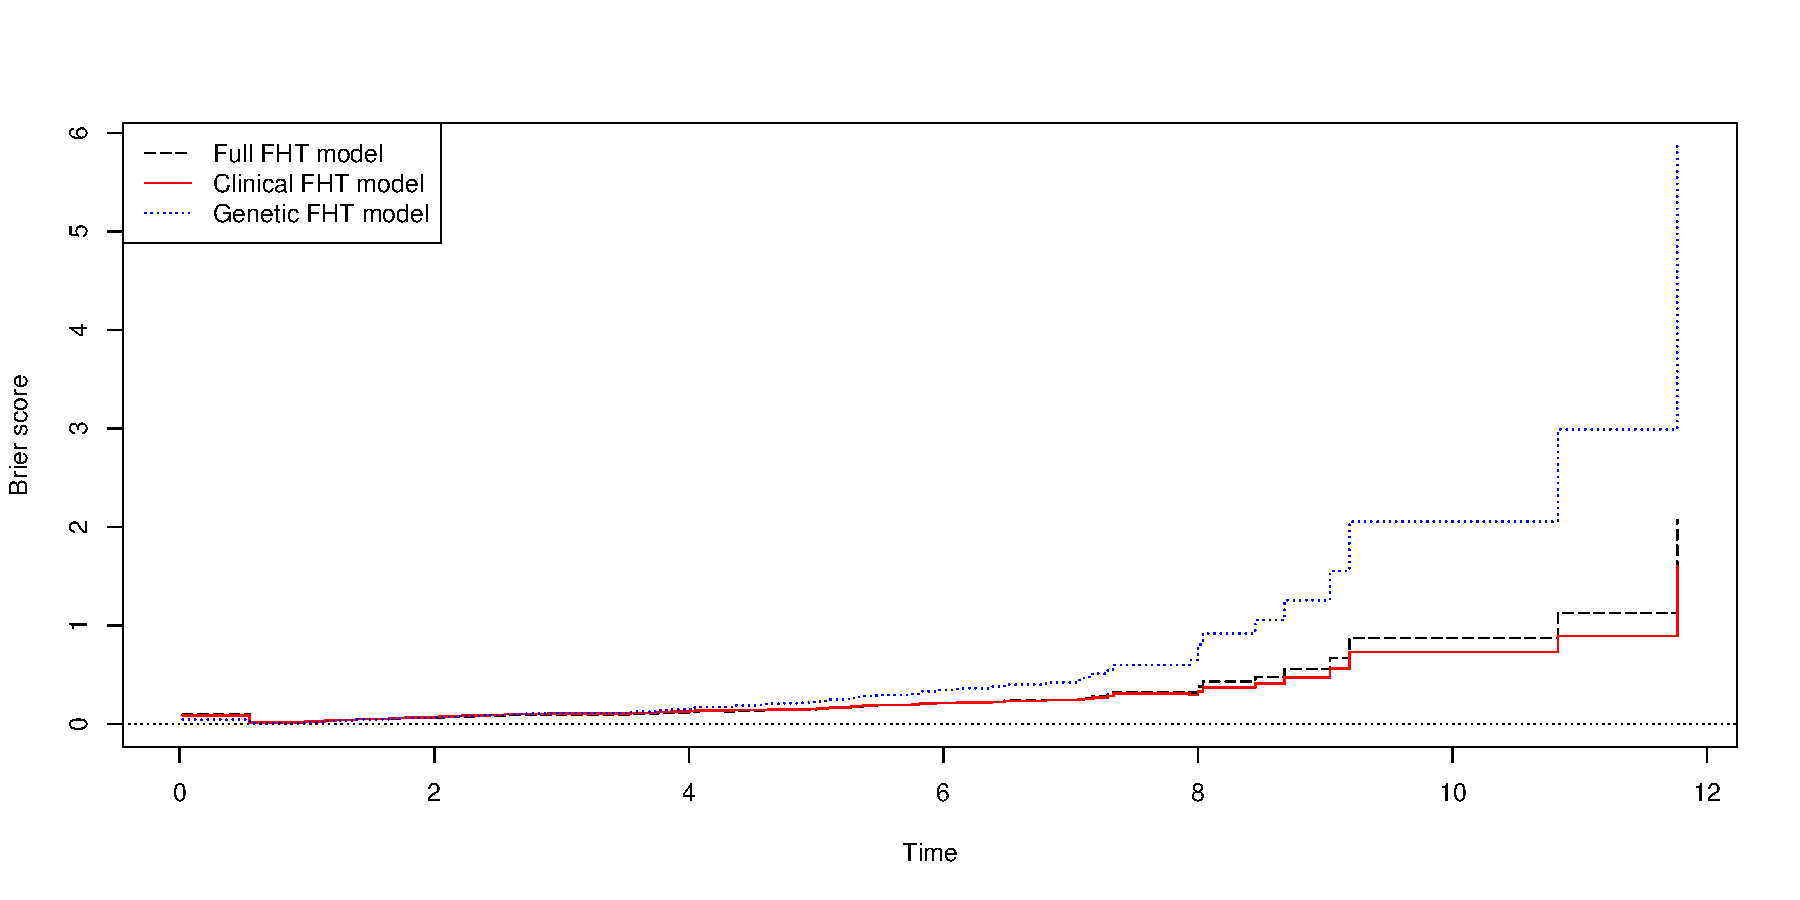
\includegraphics[scale=0.4]{brier_FHT.pdf}
\end{figure}


\subsection{Difference of deviance on the test set}
The test set in this split consists of 91 individuals, of which 14 have experienced recurrence.
We calculate the difference in deviance for the estimated FHT model, as explained in Section \ref{sec:deviance}, i.e. twice the difference of log-likelihood for an estimated model which includes covariates, versus one without.
Recall that the performance of a model is good when the difference in deviance is small (i.e. negative with a large absolute value).
We obtain a difference of deviance of -95.2.
It means that under the assumption that the FHT model is true, a lot of variation is explained by covariates.

\section{Comparing the predictive power of an FHT model with the Cox model}
To properly assess the predictive power of our estimated FHT models, we need to compare it to state of the art methods.
As we have discussed the Cox model earlier (see subsection \ref{subsec:ph-reg}), and we have implemented a boosted model, it is fitting to use \textit{CoxBoost} \citep{coxboost}.
It is an R package for estimating boosted additive predictors for the Cox model.
There exists a gradient boosted version in \textit{mboost}, but the cross-validation procedure was broken, and so we instead used \textit{CoxBoost}, which uses likelihood based boosting \citep{gamboost}.
It is a similar method that arrives at similar estimates.
In likelihood boosting, the tuning parameter is $\lambda$, and it is not directly comparable to the step length $\nu$ in gradient boosting algorithms, but we set
\begin{equation}\label{eq:lambda-nu}
    \lambda=\frac{N(1-\nu)}{\nu},
\end{equation}
as suggested in \citet{DeBin2016}.
$N$ is the number of individuals in the data set on which the estimator is applied, and $\nu$ is the step length mentioned in the various boosting algorithms in Chapter \ref{ch:boosting}, which we by convention always set to 0.1.

In the Cox model, we include all covariates when modeling the hazard function, i.e. for this neuroblastoma data set it estimates a model of the form
\begin{equation*}
    \hat{\boldeta}_{\text{CB}}=\underbrace{\hat{\beta}_{1,1}\x_1+\hat{\beta}_{1,2}\x_{2}}_{\text{clinical}}+\overbrace{\hat{\beta}_{2,1}\z_1+\ldots+\hat{\beta}_{2,9978}\z_{9978}}^{\text{genomic}},
\end{equation*}
since there are two clinical covariates and 9978 genomic ones.
In the standard boosted Cox model, all parameters are estimated in a penalized manner.
Thus there is a chance of the clinical data not being included in a final estimated model, like for FHTBoost.
However here a gene covariate will not be treated any differently than a clinical covariate, but that is something we might want.
There is also an option in \textit{CoxBoost} for specifying mandatory covariates.
These covariates will not be penalized, and hence they will be included in the final model.
We estimate both types of models on the data.

\subsection{Estimating survival probabilities in a Cox model}
To evaluate the Brier score of a survival model, we need the survival probability estimates of the model.
In a Cox model, we do not estimate the baseline hazard (see subsection \ref{subsec:ph-reg}), but this is needed to get the actual survival probability estimates.
In a Cox model which uses $\hat{\boldeta}_{\text{CB}}$, an estimate of the cumulative hazard $\hat{A}(t|\x_i,\z_i)$ is given by
\begin{equation*}
    \hat{A}(t|\x_i,\z_i)=\int_{0}^t \hz_0(s)\exp(\hat{\boldeta}_{\text{CB}})\d s=\exp(\hat{\boldeta}_{\text{CB}})\hat{A}_0(t).
\end{equation*}
To provide a survival prediction, we must therefore also estimate the baseline hazard.
This is done by estimating the \textit{cumulative} baseline hazard.
It can be done by the Breslow-Aalen estimator (see e.g. \citet{ABG}), given by
\begin{equation}
    \hat{A}_0(t)=\int_{0}^t\frac{\sum_{i=1}^N \d N_i(s)}{\sum_{i=1}^N Y_i(s)\exp \left(\hat{\boldeta}_{\text{CB}} \right)}.
\end{equation}
Here the notation $\d N_i(s)$ means the number of observed events in the infinitesimal interval $[s,s+\d s)$.
It will be zero for most intervals, but 1 at an observed event.
We do not have any tied event times in the dataset, i.e. events happening simultaneously.
If we did, we would have to make some more considerations in the above, but it is not an issue.
Further, here $Y_i(s)$ is an indicator function which is 1 if individual $i$ is at risk at time $s$, and 0 if not. 
See \ref{code:cumulative-baseline-hazard} in Appendix \ref{appendix2} for the R code we wrote to estimate this.
Given the relationship \eqref{eq:cumulative-hazard}, it follows that
\begin{equation*}
    S(t)=-\exp(A(t)),
\end{equation*}
and hence we get a \textit{CoxBoost} estimate of the survival function by
\begin{equation*}
    \hat{S}_{\text{CB}}(t)=-\exp(\hat{A}_{\text{CB}}(t))=-\exp\left(\hat{A}_0(t)\exp(\hat{\boldeta}_{\text{CB}})\right).
\end{equation*}
With all this, we can now calculate the Brier score for the Cox models as well.
\todo[inline]{Move this section to chapter 2?}
A comparison of the Brier score for the full FHT model and the Cox model can be seen in Figure \ref{fig:brier-cox-both}.
We observe that the Cox model performs better at the beginning, but at the end, the FHT model has better predictive performance.
We calculate the integrated Brier score (seen in subsection \ref{subsec:integrated-brier}).
We find that the integrated Brier score for the full FHT model is 0.0679, while the estimated CoxBoost model attains 0.0673, i.e., almost entirely the same.
For reference, the estimated FHT null model achieves 0.1226, which is almost the double.

\begin{figure}
\caption{Brier scores on a single split of the test set of the neuroblastoma data, for an estimated CoxBoost survival model and a full estimated FHT model.}
\label{fig:brier-cox-both}
\centering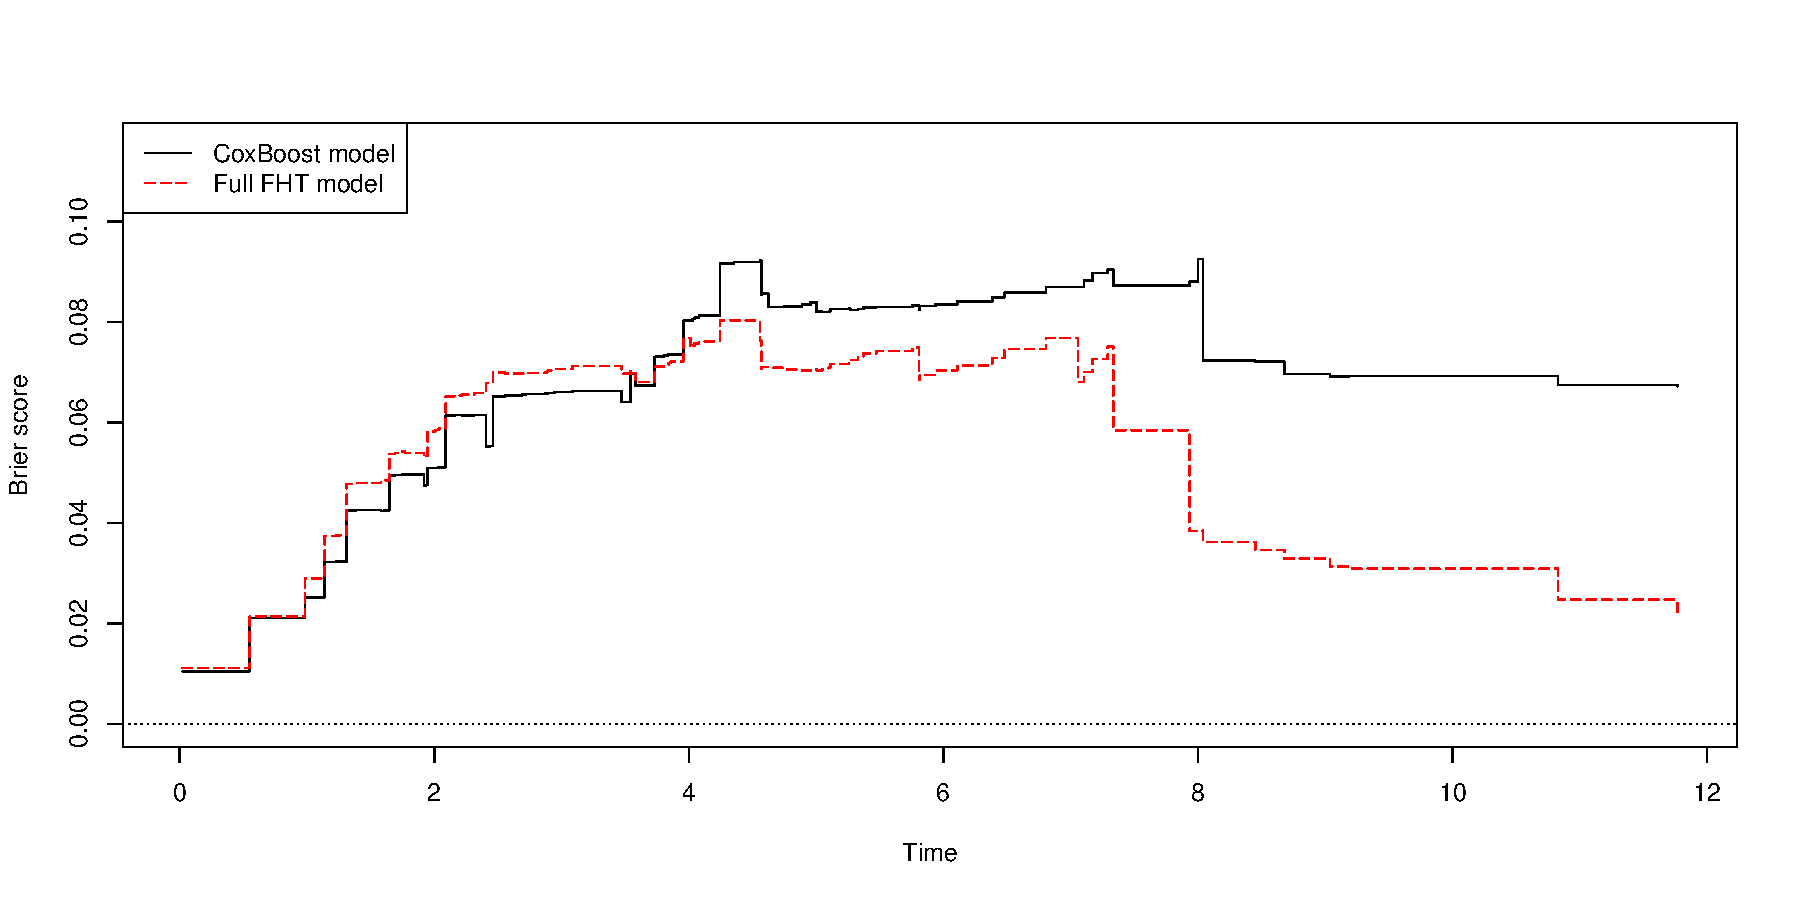
\includegraphics[scale=0.4]{brier_cox_both.pdf}
\end{figure}

%\begin{figure}
%\caption{Brier scores for Cox and Cox mandatory model.}
%\label{fig:brier-cox-mandatory}
%\centering
%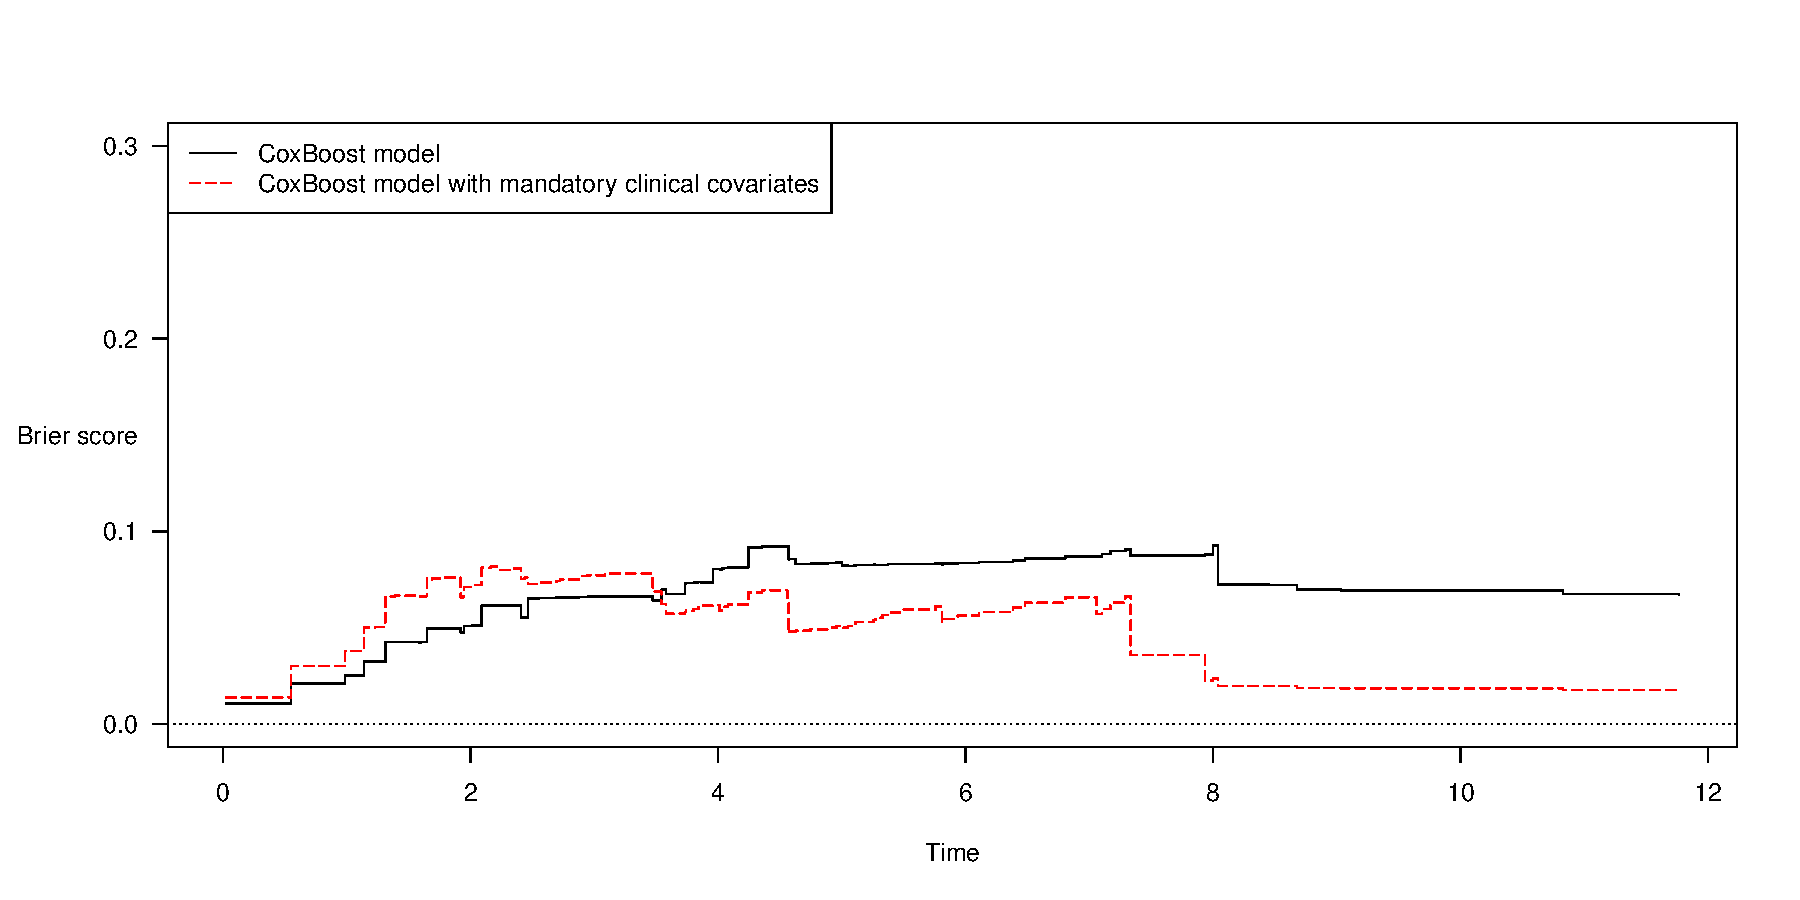
\includegraphics[scale=0.4]{brier_cox_mandatory.pdf}
%\end{figure}

%\todo[inline]{Cite these packages! I think cite(package) in R}


\section{Analysis of 100 train/test splits}
\citet{bovelstad2009} generated 50 random splits of training and test sets from the data, to see the distribution.
We now generate 100 splits of training and test sets, in the same manner.
We first estimate parameters based on the training set, and then calculate the model's difference of deviance, on the test set, using the parameters estimated on the training set.

\subsection{Difference of deviance results}
We now consider the difference of deviance across all 100 splits of training and test sets.
The main measure of interest is the mean of difference of deviance.
It is -47.217 for the full model, and -19.890 for the clinical model, and -35.533 for the genomic model.
See Figure \ref{fig:neuroblastoma-deviances} for a boxplot comparing these.
Interestingly, the median for the clinical model is -21.600, while it is 4.009 for the genomic.
So the median of the clinical model is lower than the median of the genomic model, but the \textit{mean} of the clinical model is higher than the mean of the genomic model.
Since the mean is more sensitive to extreme values, and more extreme negative values than extreme positive values will here push the mean more down, than the median will be.
It seems, therefore, that the genomic model sometimes achieves very good performance with regard to the difference of deviance.
The clinical model, on the other hand, often does not achieve that high of a deviance, but it is more stable.


\begin{figure}
\caption{Boxplot for difference in deviance for different variants of the FHT model.}
\label{fig:neuroblastoma-deviances}
\centering
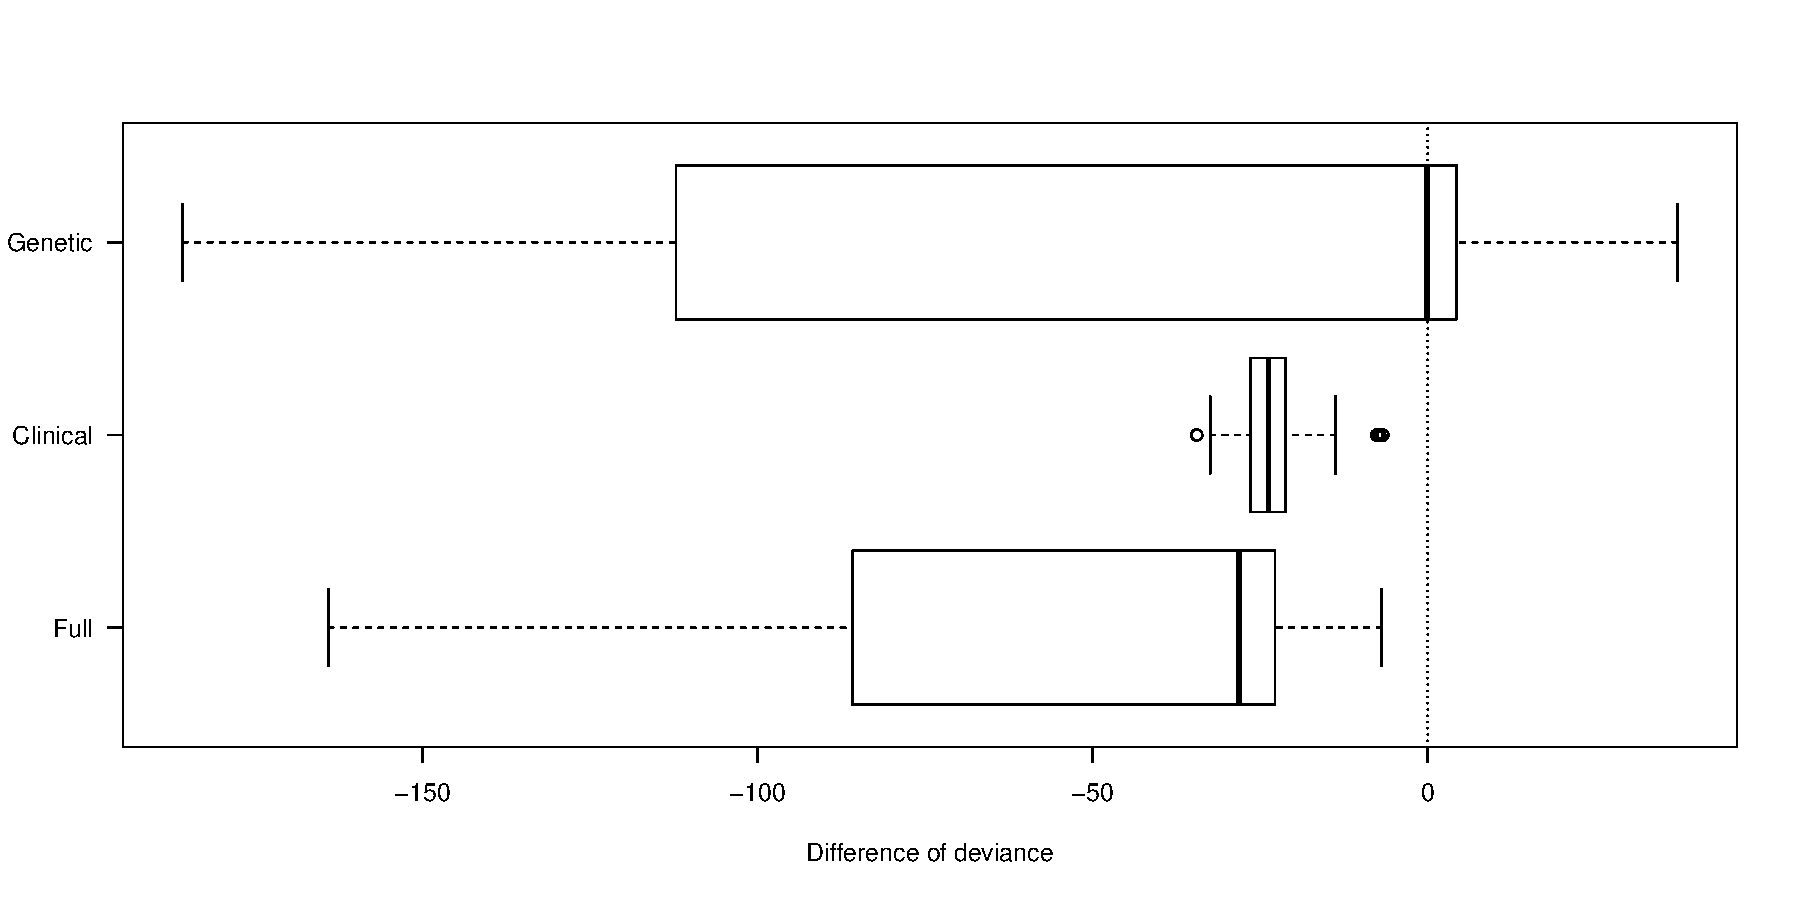
\includegraphics[scale=0.4]{deviance_FHT.pdf}
\end{figure}

%These deviances look a bit strange, at least the box for the full model, and the box for the genomic model.
%The median looks to be very strangely positioned, all the way to the right of the boxes.
%We plot histograms of these two to consider why.
%See Figure \ref {fig:neuroblastoma-deviances-histo}.
%The reason turns out to be that they are quite bimodal in their distribution.
%Both have large peaks around 0, and both have smaller and wider peaks more to the left.
%We see that the full model consistently improves performance with covariates, i.e., has a negative difference of deviance.
%This resonates with the fact that the clinical model also improves over the null model.
%However, the genomic model very often does not improve on the null model.
%Although, its most extreme values are in cases where the difference of deviance is very small, and so these are cases where the genomic model outperforms the full model.

%\begin{figure}
%\caption{Histogram of difference of deviance for the genomic model and the full model.}
%\label{fig:neuroblastoma-deviances-histo}
%\centering
%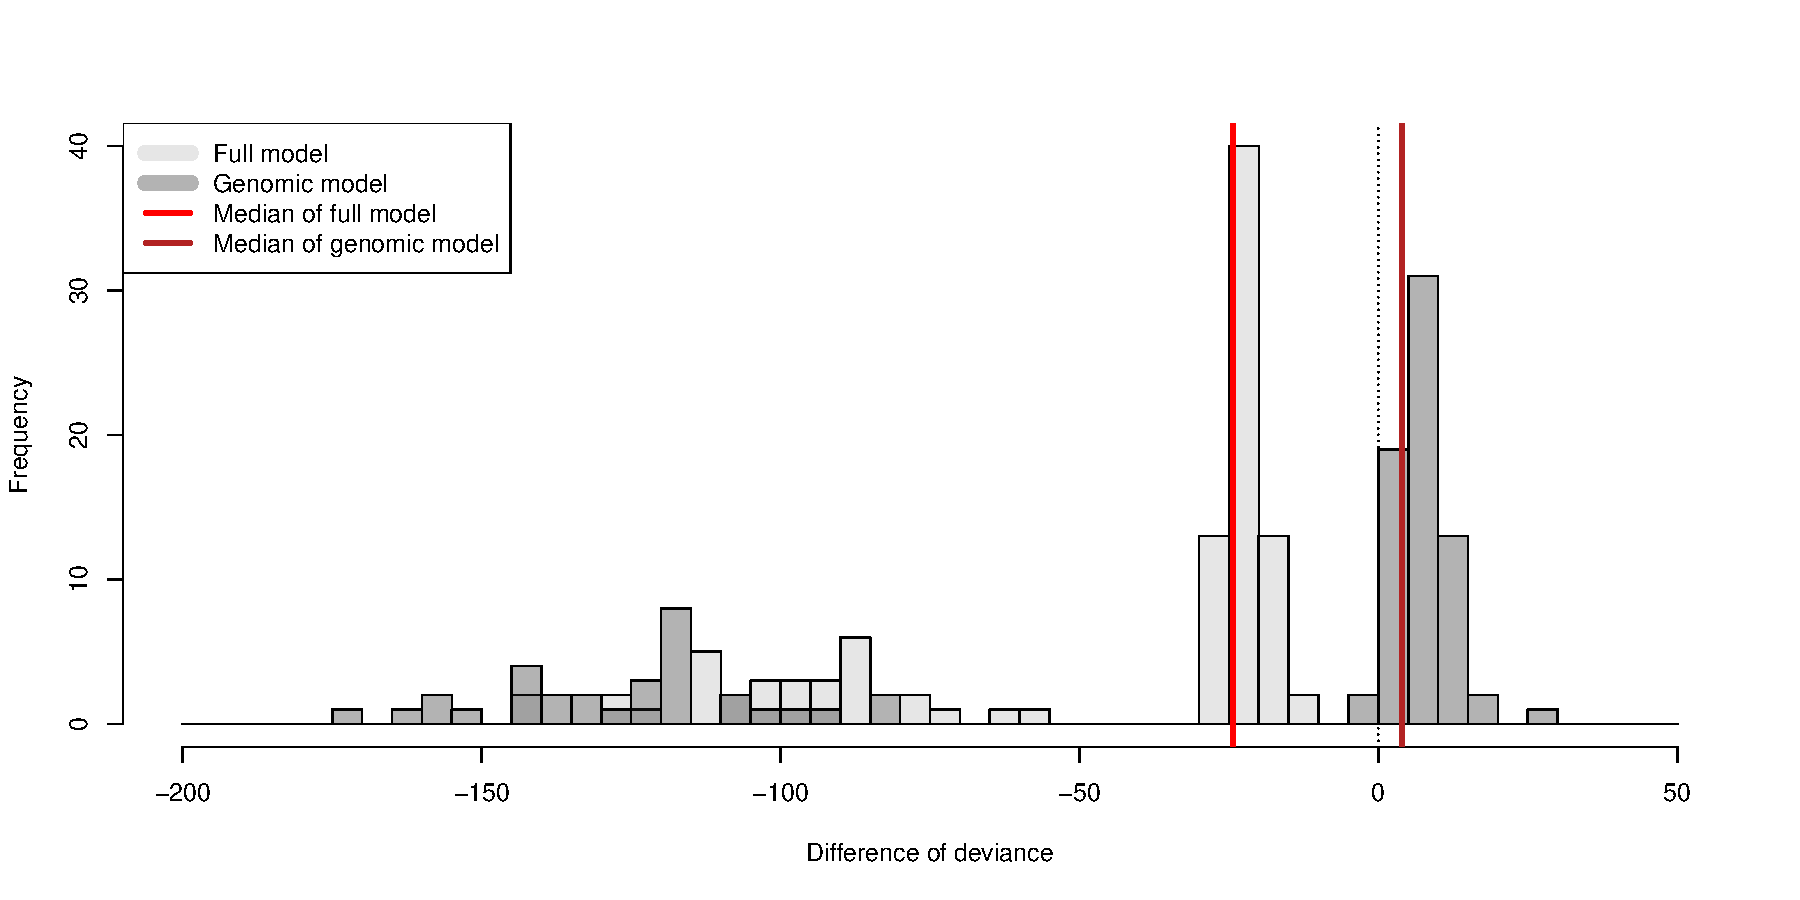
\includegraphics[scale=0.4]{deviances_histogram.pdf}
%\end{figure}


\subsection{Integrated Brier scores results}
We now calculate the integrated Brier scores for all 100 splits, for all of the mentioned methods.
A boxplot can be seen in Figure \ref{fig:neuroblastoma-integrated-brier}.
\begin{figure}
\caption{Boxplot of integrated Brier scores.}
\label{fig:neuroblastoma-integrated-brier}
\centering
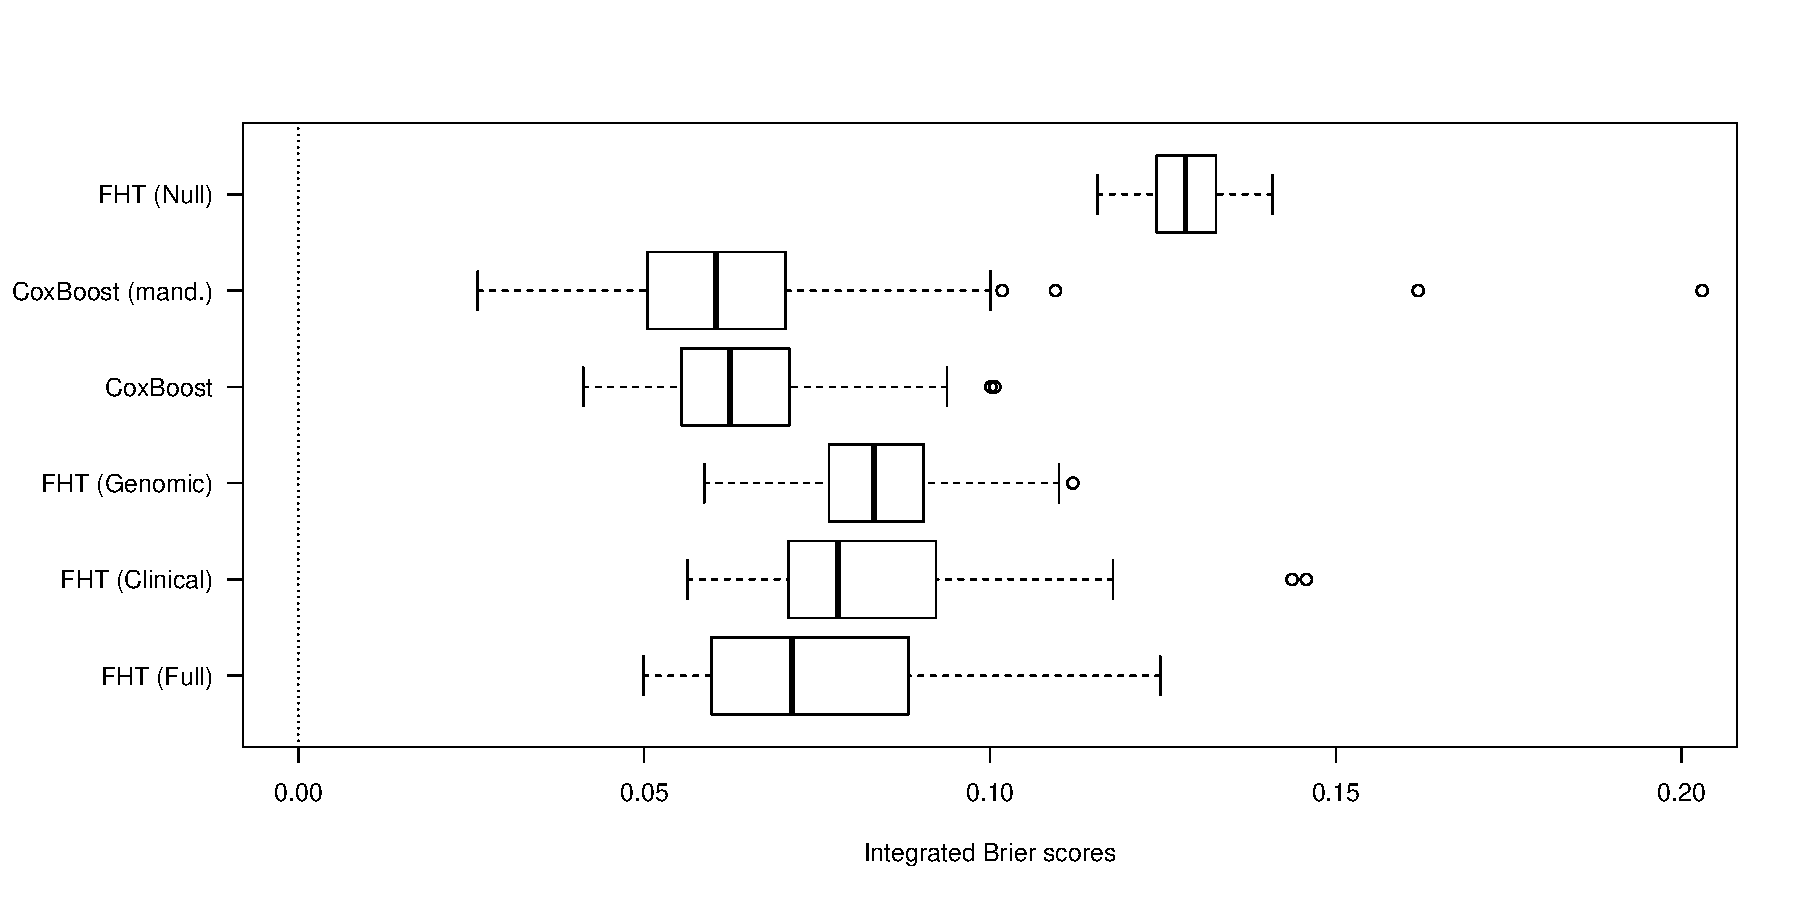
\includegraphics[scale=0.4]{integrated_brier_boxplot.pdf}
\end{figure}
For the FHT models, the full model performs best on average, with a mean of 0.0737, the clinical has 0.0791, genomic 0.0987.
For reference, the FHT null model, using only the maximum likelihood intercepts, gets 0.1185.
We might at least be relieved by the fact that the full model performs best, since it is able to incorporate all information.
This also shows that the model should be a good fit for survival data such as what we have used here.

The FHT models are, however, beaten by boosted Cox regression models.
The regular Cox model has a mean of 0.0692, while the mandatory Cox model has 0.0574.